\documentclass{beamer}
\usetheme{metropolis}

% specifications for presenter mode
%\beamerdefaultoverlayspecification{<+->}
%\setbeamercovered{transparent}

\usepackage[english]{babel}
\usepackage[utf8x]{inputenc}

%\usepackage{coloremoji}
\usepackage{layout}
\usepackage{multirow}
\usepackage{array}
\usepackage{graphicx}
\graphicspath{ {Figs/} }
\usepackage{animate}

\setbeameroption{show notes}
\setbeamertemplate{note page}[plain]
\usepackage{listings}
\usepackage{datetime}
\usepackage{url}
\usepackage{tcolorbox}
\usepackage{appendixnumberbeamer}

\usepackage{tikz}
\def\checkmark{\tikz\fill[scale=0.4](0,.35) -- (.25,0) -- (1,.7) -- (.25,.15) -- cycle;}

% math shorthand
\usepackage{bm}
\usepackage{amstext}
\usepackage{amsthm}
\usepackage{amsmath}
\usepackage{mathtools}
\newcommand{\R}{\mathbb{R}}
\newcommand{\D}{\mathcal{D}}
\newcommand{\E}{\mathbb{E}}
\newcommand{\I}{\mathbb{I}}
\newcommand{\pr}{\mathbb{P}}
\newcommand{\F}{\mathcal{F}}
\newcommand{\X}{\mathcal{X}}
\newcommand{\M}{\mathcal{M}}
\newcommand{\lik}{\mathcal{L}}

\newtheorem*{assumption*}{\assumptionnumber}
\providecommand{\assumptionnumber}{}
\makeatletter
\newenvironment{assumption}[2]
 {%
  \renewcommand{\assumptionnumber}{Assumption #1: $\mathcal{#2}$}%
  \begin{assumption*}%
  \protected@edef\@currentlabel{#1: $\mathcal{#2}$}%
 }
 {%
  \end{assumption*}
 }
\makeatother

\DeclarePairedDelimiterX{\infdivx}[2]{(}{)}{%
  #1\;\delimsize\|\;#2%
}
\newcommand{\infdiv}{D\infdivx}
\DeclarePairedDelimiter{\norm}{\lVert}{\rVert}
\DeclareMathOperator*{\argmin}{arg\,min}
\DeclareMathOperator*{\argmax}{arg\,max}

% indepndence notation macro
\newcommand\indep{\protect\mathpalette{\protect\independenT}{\perp}}
\def\independenT#1#2{\mathrel{\rlap{$#1#2$}\mkern2mu{#1#2}}}

% Bibliography
\usepackage{natbib}
\bibpunct{(}{)}{,}{a}{}{;}
\usepackage{bibentry}

\title{\normalsize Vaccine efficacy assessment under two-phase sampling based on
  the causal effects of stochastic interventions}

\author{\href{https://nimahejazi.org}{Nima Hejazi}\\[-10pt]}

\institute{
  \begin{figure}[!htb]
    \centering
    \begin{minipage}{.65\textwidth}
        Graduate Group in Biostatistics, and \\
        Center for Computational Biology, \\
        University of California, Berkeley \\[6pt]
        
\includegraphics[scale=0.12]{twitter-icon.png}
          \href{https://twitter.com/nshejazi}{nshejazi} \\
        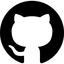
\includegraphics[scale=0.09]{github-icon.png}
          \href{https://github.com/nhejazi}{nhejazi} \\
        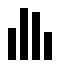
\includegraphics[scale=0.12]{homepage.png}
          \href{https://nimahejazi.org}{nimahejazi.org} \\
        
\includegraphics[scale=0.12]{pdf-icon.png}
        \href{https://bit.ly/2019\_jsm\_shift}{bit.ly/2019\_jsm\_shift} \\
        {\scriptsize joint work with David Benkeser and Mark van der Laan}
    \end{minipage}%
    \begin{minipage}{0.35\textwidth}
      \centering
      
\includegraphics[height=0.80in,width=0.80in]{ucberkeleyseal_874_540.eps}
    \end{minipage}
  \end{figure}
}

\date{Wednesday, 05 June 2019}

%%%%%%%%%%%%%%%%%%%%%%%%%%%%%%%%%%%%%%%%%%%%%%%%%%%%%%%%%%%%%%%%%%%%%%%%%%%%%%%%

\begin{document}

\begin{frame}[noframenumbering]
  \thispagestyle{empty}
  \titlepage
\end{frame}

%%%%%%%%%%%%%%%%%%%%%%%%%%%%%%%%%%%%%%%%%%%%%%%%%%%%%%%%%%%%%%%%%%%%%%%%%%%%%%%%

\begin{frame}[c]{The burden of HIV-1}

\begin{center}
\begin{itemize}
  \itemsep10pt
  \item The HIV-1 epidemic --- the facts:
    \begin{itemize}
      \item now in its fourth decade,
      \item 2.5 million new infections occurring annually worldwide,
      \item new infections outpace patients starting antiretroviral therapy.
    \end{itemize}
  \item \textit{Most efficacious} preventive vaccine: 31\% reduction rate.
  \item \textbf{Question}: How can HIV-1 vaccines be improved by modulating
    immunogenic CD4+ or CD8+ response profiles?
\end{itemize}
\end{center}

\note{
}

\end{frame}

%%%%%%%%%%%%%%%%%%%%%%%%%%%%%%%%%%%%%%%%%%%%%%%%%%%%%%%%%%%%%%%%%%%%%%%%%%%%%%%%
\begin{frame}[c]{HVTN 505 trial examined new antibody boost vaccines}

\begin{center}
\begin{itemize}
  \itemsep10pt
  \item HIV Vaccine Trials Network (HVTN) 505 vaccine efficacy RCT with
    $n = 2504$ \citep{hammer2013efficacy}.
  \item Immunogenic response profile only available for second-stage sample of
    $n = 189$ \citep{janes2017higher}.
  \item \underline{Two-phased sampling mechanism:} 100\% inclusion rate if
    HIV-1 positive in week 28; variable otherwise.
  \item \textbf{Question:} How would HIV-1 infection risk in week 28 have
    differed had immunogenic response (due to vaccine) differed?
\end{itemize}
\end{center}

\note{
\begin{itemize}
  \itemsep10pt
  \item Baseline covariates($W$): sex, age, BMI, behavioral HIV risk.
  \item Intervention(s) ($A$): post-vaccination T-cell activity markers.
  \item Outcome ($Y$): HIV-1 infection status at week 28 of tiral.
  \item \textbf{Conclusion:} Understanding which immune responses impact vaccine
    efficacy helps develop more efficacious vaccines.
  \item A vaccine effective at preventing HIV-1 acquisition would be a
    cost-effective and durable approach to halting the worldwide epidemic.
  \item Identifying vaccine-induced immune-response biomarkers that predict a
    vaccine's ability to protect individuals from HIV-1 infection is a high
    priority.
  \item The study was halted on 22 April 2013 due to absence of vaccine
    efficacy. There was no significant effect of the vaccine on the primary
    infection endpoint of HIV-1 infection between week 28 and month 24.
\end{itemize}
}

\end{frame}

%%%%%%%%%%%%%%%%%%%%%%%%%%%%%%%%%%%%%%%%%%%%%%%%%%%%%%%%%%%%%%%%%%%%%%%%%%%%%%%%

\begin{frame}[c]{Two-phase sampling censors the complete data structure}

\begin{center}
\begin{itemize}
  \itemsep10pt
  \item Complete, unobserved data $X = (W, A, Y) \sim P_0^X \in
    \mathcal{M}^X_{NP}$, as per the full HVTN 505 RCT
    \citep{hammer2013efficacy}:
    \vspace{1em}
    \begin{itemize}
      \itemsep8pt
      \item $W$ --- baseline covariates: sex, age, BMI, behavioral HIV risk,
      \item $A$ --- intervention: immune response profile for CD4 and CD8,
      \item $Y$ --- outcome of interest: HIV-1 infection status by week 28.
    \end{itemize}
  \item Observed data $O = (\Delta, \Delta X) = (W, \Delta, \Delta A, Y)$,
    $\Delta \in \{0,1\}$, as per the second-stage sample of
    \cite{janes2017higher}.
\end{itemize}
\end{center}

\note{
  \begin{itemize}
    \item $P_0^X$ --- true (unknown) distribution of the full data $X$,
    \item $\mathcal{M}^X_{NP}$ --- nonparametric statistical model.
  \end{itemize}
}

\end{frame}

%%%%%%%%%%%%%%%%%%%%%%%%%%%%%%%%%%%%%%%%%%%%%%%%%%%%%%%%%%%%%%%%%%%%%%%%%%%%%%%%

\begin{frame}[c]{Stochastic interventions define the causal effects of shifts}

\begin{center}
\begin{itemize}
  \itemsep10pt
  \item Causal estimand: counterfactual mean of HIV-1 infection under a
    \textit{shifted} immunogenic response distribution.
  \item \cite{diaz2012population, diaz2018stochastic}: \textit{Shift}
    interventions?
     \begin{equation*}\label{shift_intervention}
       d(a, w) =
         \begin{cases}
           a + \delta, & \text{if plausible} \\
           a, & \text{otherwise}
         \end{cases}
     \end{equation*}
  \item \cite{diaz2012population, diaz2018stochastic} give a statistical target
    parameter and influence function for the complete data case.
  \item \textbf{Challenge:} parameter estimation requires conditional density
    estimation. Nonparametric options?
\end{itemize}
\end{center}

\note{
  \begin{itemize}
    \item For HVTN 505, $\psi_{0,d}$ is the counterfactual risk of HIV-1
      infection, had the observed value of the immune response been modifed to
      originate from the distribution of the rule $d(A,W)$.
    \item Several different ways to consider stochastic interventions.
    \item Starts with Mark and Ivan's simple stochastic shift.
    \item Extensions to modified treatment policies.
    \item The new value of $A$ may be denoted $A^{\star} \sim
      G^{\star}(\cdot \mid W)$, where $A^{\star} = d(W, U^{\star})$ for a rule
      $d$ and random error $U^{\star}$.
  \end{itemize}
}

\end{frame}

%%%%%%%%%%%%%%%%%%%%%%%%%%%%%%%%%%%%%%%%%%%%%%%%%%%%%%%%%%%%%%%%%%%%%%%%%%%%%%%%

\begin{frame}[c]{HIV-1 risk under stochastically shifted immune responses}

\centering
\animategraphics[loop,controls,scale=0.13]{10}{shift_animation-}{0}{6}

\note{
}

\end{frame}

%%%%%%%%%%%%%%%%%%%%%%%%%%%%%%%%%%%%%%%%%%%%%%%%%%%%%%%%%%%%%%%%%%%%%%%%%%%%%%%%

\begin{frame}[c]{Efficient estimators in spite of two-phase sampling}

\begin{center}
\begin{itemize}
  \itemsep10pt
  \item What if sampling mechanism $\pi_0(Y, W) = \pr(\Delta=1 \mid Y,W)$
    is not known by design? Nonparametric estimation of $\pi_0(Y, W)$?
  \item Building on \cite{rose2011targeted2sd}, we provide
    \begin{itemize}
      \itemsep4pt
      \item asymptotically linear and nonparametric-\textit{efficient}
        estimators;
      \item multiply \textit{robust}, with 2 forms of double robustness;
      \item Gaussian limiting distributions and Wald-type CIs.
    \end {itemize}
  \item New open source software for deploying such estimators:
    \begin{itemize}
      \itemsep4pt
      \item \url{https://github.com/nhejazi/haldensify} (densities)
      \item \url{https://github.com/nhejazi/txshift} (AIPW, TMLE)
      \item \url{https://github.com/tlverse/tmle3shift} (TMLE)
    \end {itemize}
\end{itemize}
\end{center}

\note{
\begin{itemize}
  \itemsep10pt
  \item \textbf{Asymptotic linearity:}
    \begin{equation*}
      \Psi(P_n^{\star}) - \Psi(P_0^X) = \frac{1}{n} \sum_{i = 1}^{n}
      D(P_0^X)(X_i) + o_P\left(\frac{1}{\sqrt{n}}\right)
    \end{equation*}
  \item \textbf{Gaussian limiting distribution:}
    \begin{equation*}
      \sqrt{n}(\Psi(P_n^{\star}) - \Psi(P_0^X)) \to N(0, Var(D(P_0^X)(X)))
    \end{equation*}
  \item \textbf{Statistical inference:}
    \begin{equation*}
      \text{Wald-type confidence interval}:
      \Psi(P_n^{\star}) \pm z_{\alpha} \cdot \frac{\sigma_n}{\sqrt{n}},
    \end{equation*}
    where $\sigma_n^2$ is computed directly via
    $\sigma_n^2 = \frac{1}{n} \sum_{i = 1}^{n} D^2(\cdot)(X_i)$.
\end{itemize}
}

\end{frame}

%%%%%%%%%%%%%%%%%%%%%%%%%%%%%%%%%%%%%%%%%%%%%%%%%%%%%%%%%%%%%%%%%%%%%%%%%%%%%%%%

\begin{frame}[c]{How does this help in fighting the HIV-1 epidemic? CD4+}

\vspace{-2em}
\begin{figure}[H]
  \centering
  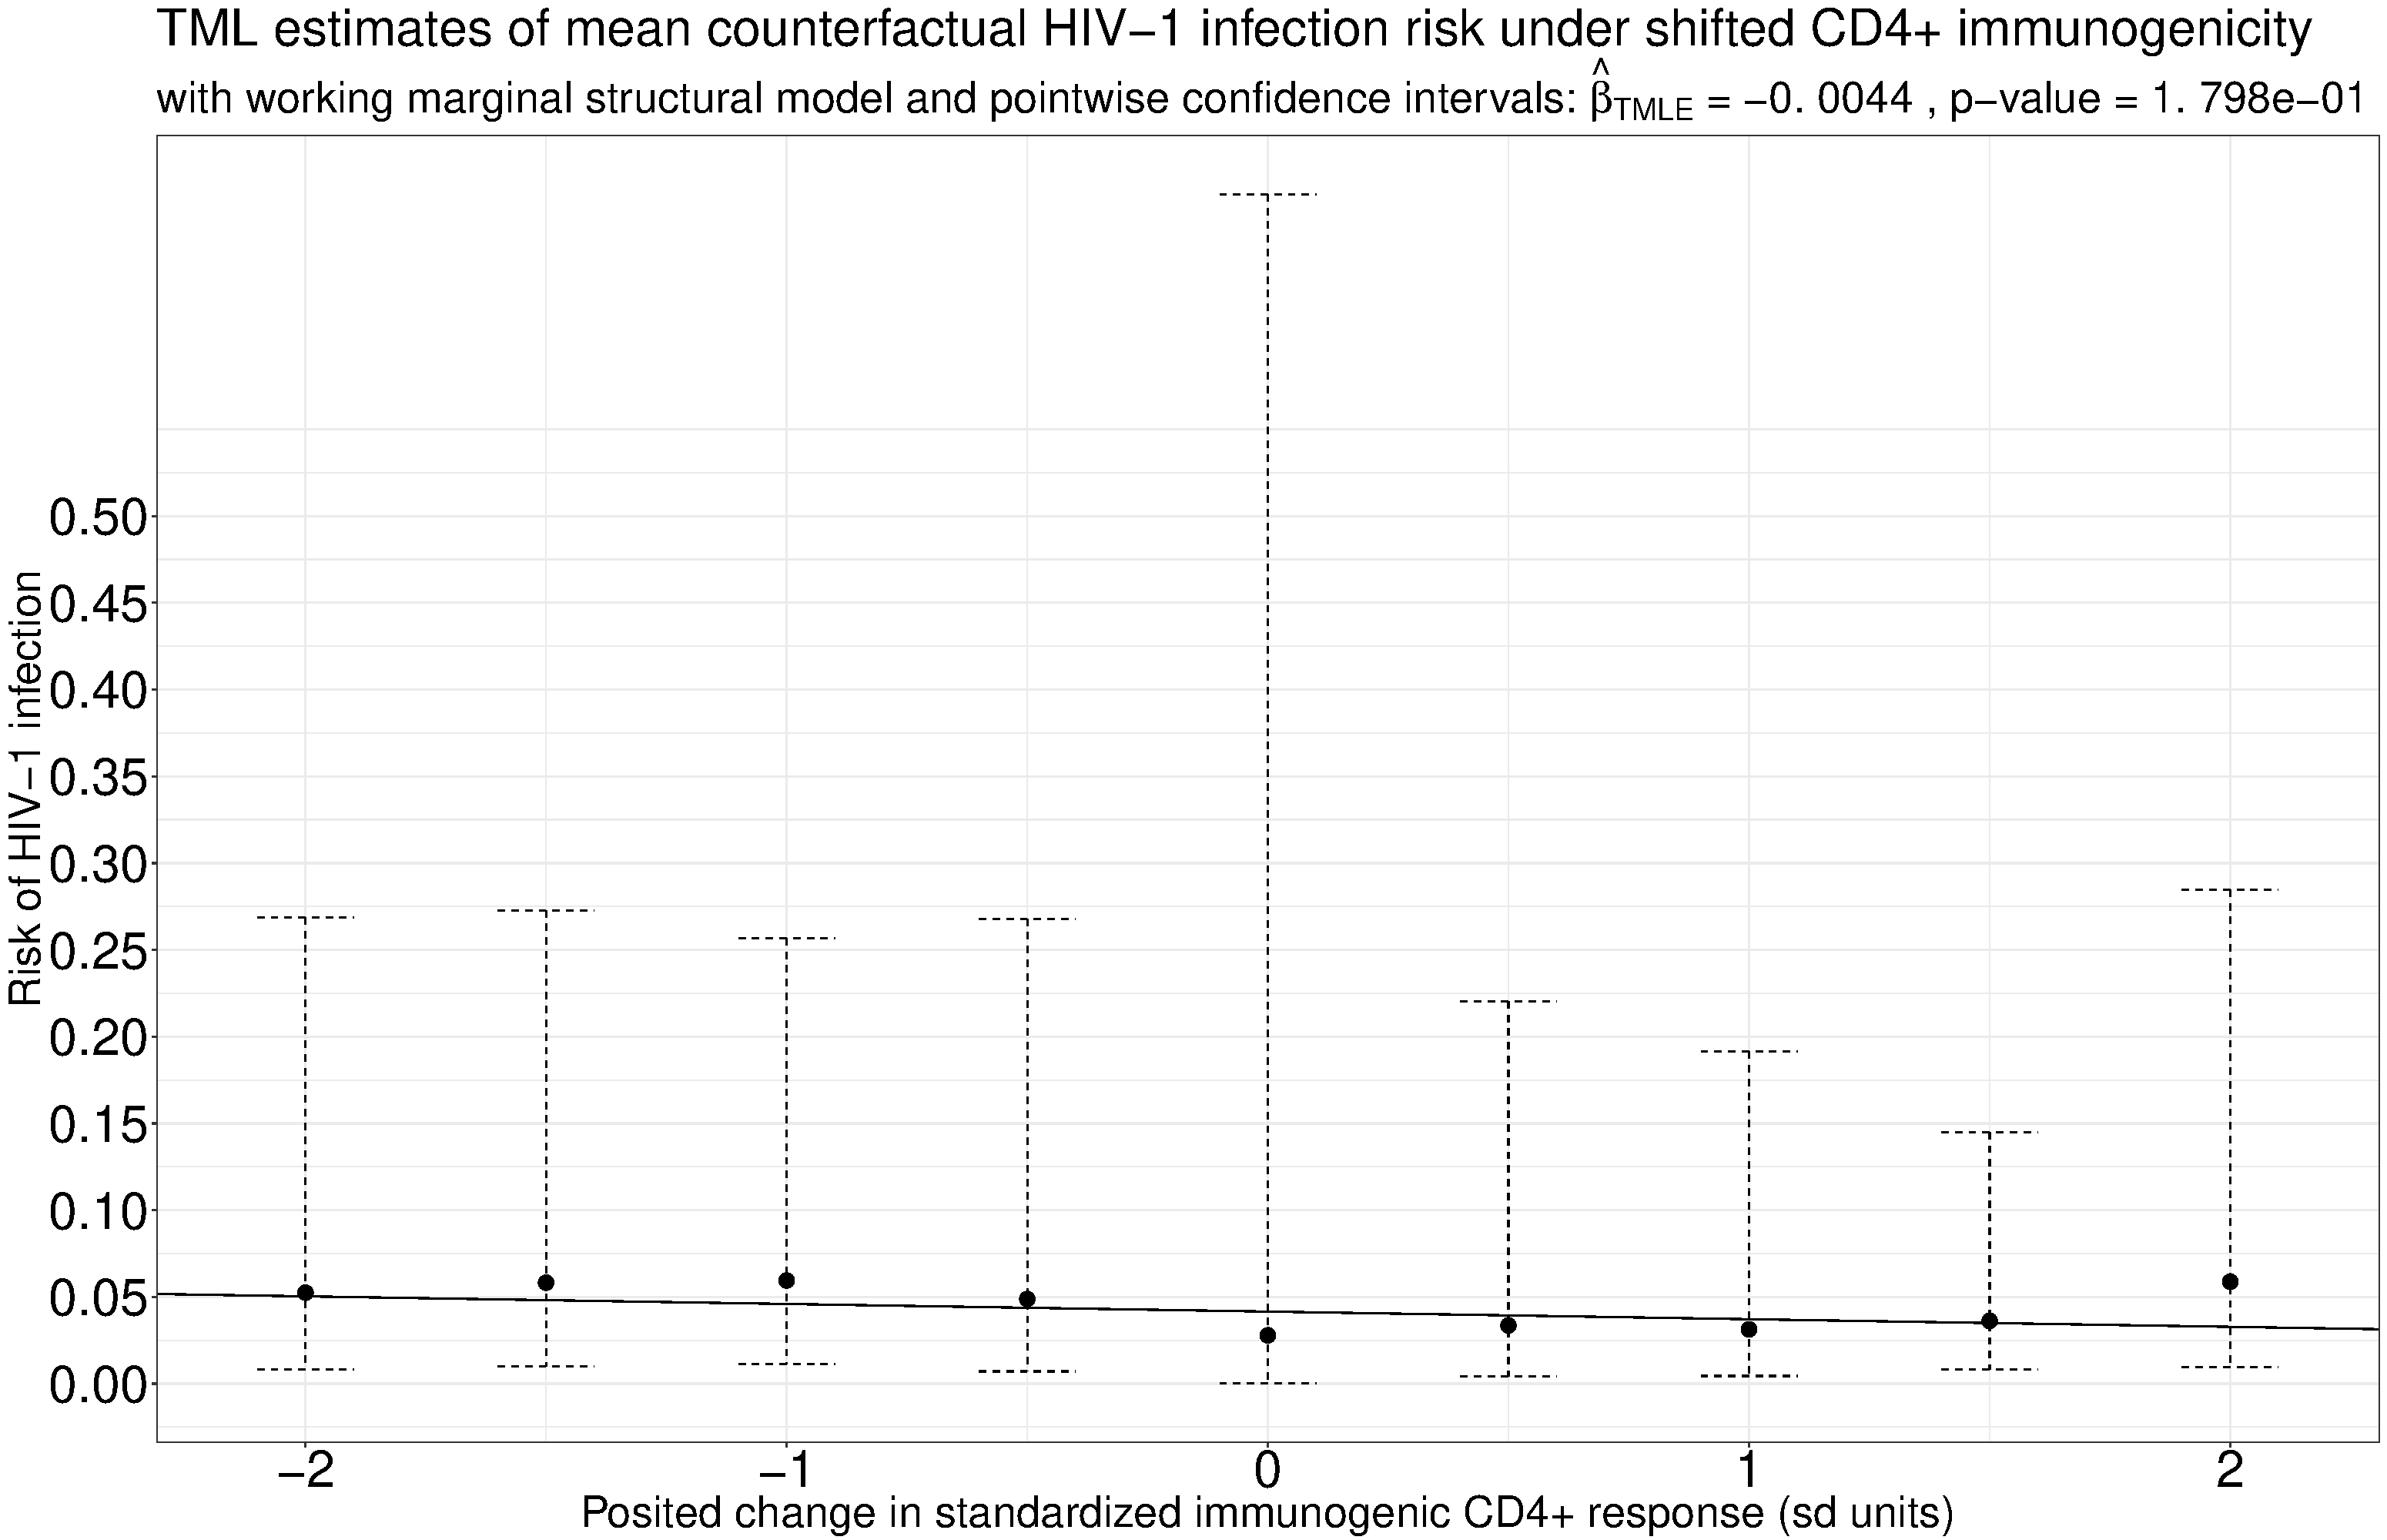
\includegraphics[scale=0.21]{cd4_msm_tmle_summary}
  \caption{
    Analysis of HIV-1 risk as a function of CD4+ immunogenicity, using
    \texttt{R} package \texttt{txshift}
    (\url{https://github.com/nhejazi/txshift}.)
  }
\end{figure}

\note{
}

\end{frame}

%%%%%%%%%%%%%%%%%%%%%%%%%%%%%%%%%%%%%%%%%%%%%%%%%%%%%%%%%%%%%%%%%%%%%%%%%%%%%%%%

\begin{frame}[c]{How does this help in fighting the HIV-1 epidemic? CD8+}

\vspace{-2em}
\begin{figure}[H]
  \centering
  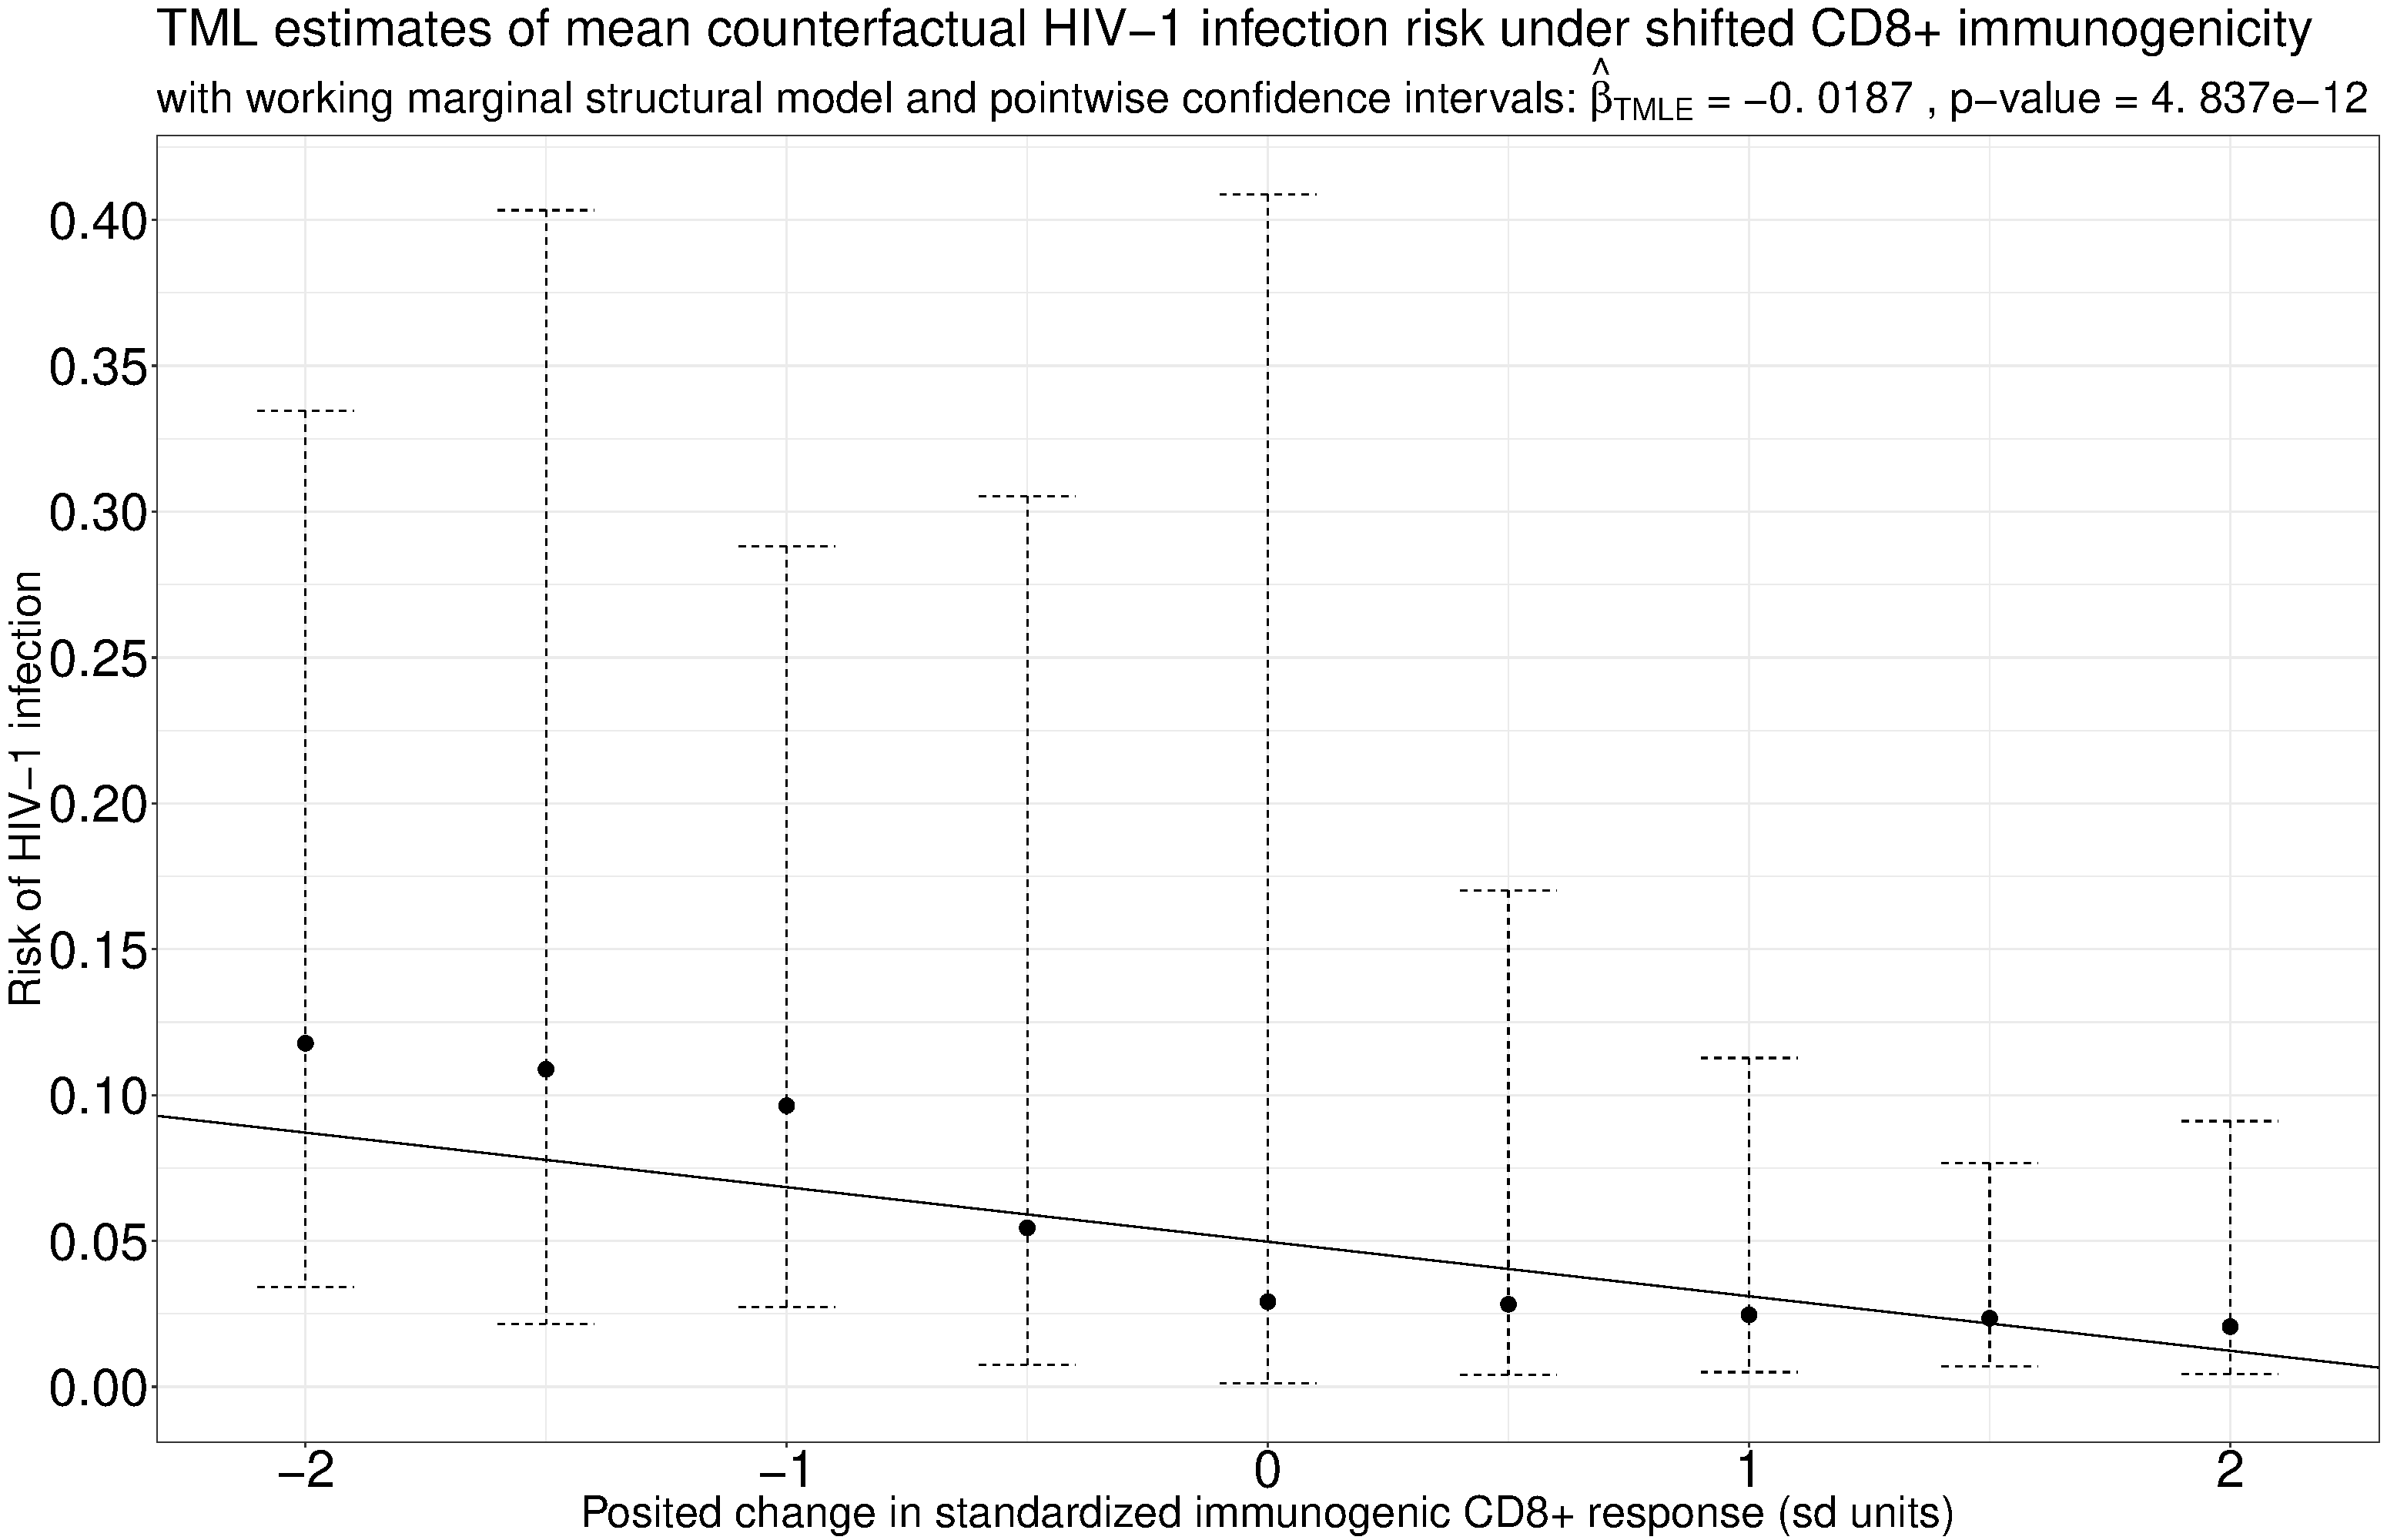
\includegraphics[scale=0.21]{cd8_msm_tmle_summary}
  \caption{
    Analysis of HIV-1 risk as a function of CD8+ immunogenicity, using
    \texttt{R} package \texttt{txshift}
    (\url{https://github.com/nhejazi/txshift}.)
  }
\end{figure}

\note{
}

\end{frame}

%%%%%%%%%%%%%%%%%%%%%%%%%%%%%%%%%%%%%%%%%%%%%%%%%%%%%%%%%%%%%%%%%%%%%%%%%%%%%%%%

% don't want dimming with references
\setbeamercovered{}
\beamerdefaultoverlayspecification{}

\begin{frame}[c,allowframebreaks]{}

\scriptsize
\bibliographystyle{apalike}
\bibliography{references}

\end{frame}

%%%%%%%%%%%%%%%%%%%%%%%%%%%%%%%%%%%%%%%%%%%%%%%%%%%%%%%%%%%%%%%%%%%%%%%%%%%%%%%%

\begin{frame}[c]{Thank you.}

\large
Slides: \href{http://bit.ly/2019\_jsm\_shift}{bit.ly/2019\_jsm\_shift}
  \quad

\includegraphics[height=4mm]{Figs/cc-zero.png}

\vspace{2mm}
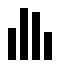
\includegraphics[scale=0.14]{homepage.png} \url{https://nimahejazi.org}

\vspace{2mm}
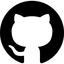
\includegraphics[scale=0.11]{github-icon.png}
  \url{https://github.com/nhejazi}

\vspace{2mm}

\includegraphics[scale=0.14]{twitter-icon.png}
  \url{https://twitter.com/nshejazi}

\end{frame}

%%%%%%%%%%%%%%%%%%%%%%%%%%%%%%%%%%%%%%%%%%%%%%%%%%%%%%%%%%%%%%%%%%%%%%%%%%%%%%%%

\end{document}
